\documentclass[a4paper, 12pt]{article}        % General format
%\documentclass[a4paper, 14pt]{extarticle}    % Advanced format

%%%% Charset
\usepackage{cmap}                             % Make PDF files searchable and copyable
\usepackage[utf8x]{inputenc}                  % Accept different input encodings
\usepackage[T2A]{fontenc}                     % Russian font
\usepackage[russian]{babel}                   % Multilingual support (T2A)

%%%% Graphics
\usepackage[dvipsnames]{xcolor}               % Driver-independent color extensions
\usepackage{graphicx}                         % Enhanced support for graphics
\usepackage{wrapfig}                          % Produces figures which text can flow around

%%%% Graphs
\usepackage{tikz}                             % Creating graphics programmatically
\usetikzlibrary{arrows}                       % Arrows for tikz

%%%% Math
\usepackage{amsmath}                          % American Mathematical Society (AMS) math facilities
\usepackage{amsfonts}                         % fonts from the AMS
\usepackage{amssymb}                          % additional math symbols

%%%% Typography (don't forget about cm-super)
\usepackage{microtype}                        % subliminal refinements towards typographical perfection
\linespread{1.3}                              % line spacing
\usepackage[left=2.5cm, right=1.5cm, top=2.5cm, bottom=2.5cm]{geometry}
\setlength{\parindent}{0pt}                   % we don't want any paragraph indentation
\usepackage{parskip}                          % add distance between paragraphs

%%%% Tables
\usepackage{tabularx}                         % Enhanced tables
\usepackage{multirow}                         % For tabular
\usepackage{hhline}                           % For tabular

%%%% Other
\usepackage{url}                              % Verbatim with URL-sensitive line breaks
\usepackage{fancyvrb}                         % Sophisticated verbatim text
\setcounter{secnumdepth}{5}                   % Turn on subsection numbering

%------------------------------------------------------------------------------
\usepackage{listings}                         % typeset source code listings

% Цвета для кода
\definecolor{mygreen}{HTML}{3F7F5F}           % color values Red, Green, Blue
\definecolor{mylilas}{RGB}{170,55,241}

% Настройки отображения кода
\lstset{language=Matlab,%
    %basicstyle=\color{red},
    breaklines    =  true,                    % Перенос длинных строк
    morekeywords  =  {matlab2tikz},           %
    keywordstyle  =  \color{blue},            %
    morekeywords  =  [2]{1},                  %
    keywordstyle  =  [2]{\color{black}},      %
    identifierstyle= \color{black},           %
    stringstyle   =  \color{mylilas},         %
    commentstyle  =  \color{mygreen},         %
    showstringspaces=false,                   % don't mark spaces in strings
    frame         =  tblr                     % draw a frame at all sides of the code block
    rulecolor     =  \color{frame},           % Цвет рамки
    tabsize       =  2,                       % tab space width
    showstringspaces=false,                   % don't mark spaces in strings
    numbers       =  left,                    %
    numberstyle   =  {\tiny \color{black}},   % size of the numbers
    numbersep     =  9pt,                     % this defines how far the numbers are from the text
    emph          =  [1]{for,end,break},      %
    emphstyle     =  [1]\color{red},          %some words to emphasise
    %emph         =  [2]{word1,word2},        %
    %emphstyle    =  [2]{style},              %
    extendedchars =  true,                    % Для отображения русского языка
    literate=
        {Ö}{{\"O}}1                    {Ä}{{\"A}}1                    {Ü}{{\"U}}1
        {ß}{{\ss}}1                    {ü}{{\"u}}1                    {ä}{{\"a}}1
        {ö}{{\"o}}1                    {~}{{\textasciitilde}}1        {а}{{\selectfont\char224}}1
        {б}{{\selectfont\char225}}1    {в}{{\selectfont\char226}}1    {г}{{\selectfont\char227}}1
        {д}{{\selectfont\char228}}1    {е}{{\selectfont\char229}}1    {ё}{{\"e}}1
        {ж}{{\selectfont\char230}}1    {з}{{\selectfont\char231}}1    {и}{{\selectfont\char232}}1
        {й}{{\selectfont\char233}}1    {к}{{\selectfont\char234}}1    {л}{{\selectfont\char235}}1
        {м}{{\selectfont\char236}}1    {н}{{\selectfont\char237}}1    {о}{{\selectfont\char238}}1
        {п}{{\selectfont\char239}}1    {р}{{\selectfont\char240}}1    {с}{{\selectfont\char241}}1
        {т}{{\selectfont\char242}}1    {у}{{\selectfont\char243}}1    {ф}{{\selectfont\char244}}1
        {х}{{\selectfont\char245}}1    {ц}{{\selectfont\char246}}1    {ч}{{\selectfont\char247}}1
        {ш}{{\selectfont\char248}}1    {щ}{{\selectfont\char249}}1    {ъ}{{\selectfont\char250}}1
        {ы}{{\selectfont\char251}}1    {ь}{{\selectfont\char252}}1    {э}{{\selectfont\char253}}1
        {ю}{{\selectfont\char254}}1    {я}{{\selectfont\char255}}1    {А}{{\selectfont\char192}}1
        {Б}{{\selectfont\char193}}1    {В}{{\selectfont\char194}}1    {Г}{{\selectfont\char195}}1
        {Д}{{\selectfont\char196}}1    {Е}{{\selectfont\char197}}1    {Ё}{{\"E}}1
        {Ж}{{\selectfont\char198}}1    {З}{{\selectfont\char199}}1    {И}{{\selectfont\char200}}1
        {Й}{{\selectfont\char201}}1    {К}{{\selectfont\char202}}1    {Л}{{\selectfont\char203}}1
        {М}{{\selectfont\char204}}1    {Н}{{\selectfont\char205}}1    {О}{{\selectfont\char206}}1
        {П}{{\selectfont\char207}}1    {Р}{{\selectfont\char208}}1    {С}{{\selectfont\char209}}1
        {Т}{{\selectfont\char210}}1    {У}{{\selectfont\char211}}1    {Ф}{{\selectfont\char212}}1
        {Х}{{\selectfont\char213}}1    {Ц}{{\selectfont\char214}}1    {Ч}{{\selectfont\char215}}1
        {Ш}{{\selectfont\char216}}1    {Щ}{{\selectfont\char217}}1    {Ъ}{{\selectfont\char218}}1
        {Ы}{{\selectfont\char219}}1    {Ь}{{\selectfont\char220}}1    {Э}{{\selectfont\char221}}1
        {Ю}{{\selectfont\char222}}1    {Я}{{\selectfont\char223}}1    {і}{{\selectfont\char105}}1
        {ї}{{\selectfont\char168}}1    {є}{{\selectfont\char185}}1    {ґ}{{\selectfont\char160}}1
        {І}{{\selectfont\char73}}1     {Ї}{{\selectfont\char136}}1    {Є}{{\selectfont\char153}}1
        {Ґ}{{\selectfont\char128}}1
}

\usepackage{caption}                          % Для настройки заголовка кода
\DeclareCaptionFont{white}{\color{сaptiontext}}
\DeclareCaptionFormat{listing}{\parbox{\linewidth}{\colorbox{сaptionbk}{\parbox{\linewidth}{#1#2#3}}\vskip-4pt}}
%\captionsetup[lstlisting]{format=listing,labelfont=white,textfont=white}
\renewcommand{\lstlistingname}{Листинг}       % Переименование Listings в нужное именование структуры
%------------------------------------------------------------------------------

\begin{document}

\begin{titlepage}
\thispagestyle{empty}

\begin{center}
Санкт-Петербургский политехнический университет Петра Великого\\
Институт компьютерных наук и технологий\\*
Кафедра компьютерных систем и программных технологий\\*
\hrulefill
\end{center}

\vspace{15em}

\begin{center}
\textsc{\textbf{Курсовая работа}}
\vspace{1em}

Дисциплина: \textbf{Моделирование вычислительных систем}
\vspace{2em}

Тема: \textbf{Моделирование работы транспортного цеха}
\end{center}

\vspace{16em}

\begin{flushleft}
Выполнил студент гр. 63501/3 \hrulefill С.А. Мартынов \\
\vspace{1.5em}
Руководитель, к.т.н.,доц. \hrulefill А.Г. Сиднев\\
\end{flushleft}

\vspace{\fill}

\begin{center}
Санкт-Петербург \\
2015
\end{center}

\end{titlepage}
\setcounter{page}{2}                            % Титульная страница
\tableofcontents

%------------------------------------------------------------------------------

%\input{text}                                 % Текст
\newpage
\section*{Постановка задачи}
\addcontentsline{toc}{section}{Постановка задачи}

Транспортный цех объединения обслуживает три филиала А, В и С. Грузовики перевозят изделия из А в В и из В в С, возвращаясь затем в А без груза. Погрузка в А занимает 20 минут, переезд из А в В длится 30 минут, разгрузка и погрузка в В -- по 20 минут, переезд в С -- 30 минут, разгрузка в С -- 20 мин и переезд в А -- 20 мин. Если к моменту погрузки в А и В отсутствуют изделия, грузовики уходят дальше по маршруту. Изделия в А выпускаются партиями по 1000 штук через 20$\pm$3 минуты, в В -- такими же партиями через 20$\pm$5 минут. На линии работает 8 грузовиков, каждый перевозит по 1000 изделий. В начальный момент все грузовики находятся в А.

Смоделировать работу транспортного цеха в течение 1000 часов. Определить частоту пустых перегонов грузовиков между А и В, В и С и сравнить с характеристиками, полученными при равномерном начальном распределении грузовиков между филиалами и операциями. Определить средне время цикла грузовика.

\newpage
\section{Моделирование в среде GPSS}

\subsection{Построение GPSS-модели}

Из условий задачи, входным потоком модели являются изделия, производимые в филиалах A и B. Выходным потоком -- грузовики, покидающие филиал A.

Рассмотрим работу грузовиков в стационарном режиме (т.е. спустя некоторое время от начала процесса) без пустых перегонов. Тогда один грузовик выполняет полный список задач (начиная с выезда из филиала A и заканчивая возвращение в него же) за 160 минут, т.е. время переездов 30 + 30 + 20 = 80 и время разгрузочно-погрузочных работ 20 + 20 + 20 + 20 = 80.

Грузовику требуется 160 минут на перевозку двух партий изделий, т.о. на перевозку одной партии в среднем требуется 80 минут. По условиям задачи у нас 8 грузовиков, тогда одну партию можно перевезти за 80/8 = 10 минут (в среднем).

Теперь рассмотрим производство. Филиал А выпускает одну парти деталей (в среднем) за 20 минут. Филиал B выпускает тот же объём за то же время. Таким образом, каждые 10 минут (в среднем) филиалы способны выдавать по одной партии, и это время идеально подходит под среднюю загрузку транспортного цеха из 8 грузовиков. Очевидно, что если что-то откланяется от идеально-средней схемы, возникнут пустые перегоны, грузовики не будут успевать перевозить груз и он будет скапливаться в филиалах.

Построим модель (Листинг 1) в системе моделирования GPSS по следующим исходным данным:
\begin{itemize}
\item Выпуск изделий в филиале А -- 20$\pm$3 минут
\item Выпуск изделий в филиале В -- 20$\pm$5 минут
\item Количество грузовиков в работе -- 8 единиц
\item Время погрузки в А -- 20 минут
\item Время погрузки в В -- 20 минут
\item Время разгрузки в В -- 20 минут
\item Время разгрузки в С -- 20 минут
\item Время переезда из А в В -- 30 минут
\item Время переезда из В в С -- 30 минут
\item Время переезда из С в А -- 20 минут
\item Вместимость одного грузовика -- 1000 изделий
\item Объем одной партии -- 1000 изделий
\item Время работы транспортного цеха -- 60000 минут (1000 часов)
\end{itemize}

\lstinputlisting[language={},caption={Наивная реализация модели}]{res/prog1.gpss}

Результаты её работы представлены в листинге 2.

\lstinputlisting[language={},caption={Отчёт по работе наивной реализации модели}]{res/prog1.report}

В 60-й строке видно, что за всё время работы было совершено 32 пустых проезда (на 13-ю строку обращать внимание не стоит, она только показывает сколько раз это значение было перевычислено). Очевидно, большая часть таких проездов совершается в самом начале, когда на маршрут выпускаются сразу все 8 машин, при этом первые партии продукции появятся только через 20 минут после этого. Мы можем выпускать машины с интервалом раз в 10 минут, и делать это только на 20-й минуте. Для этого нужно изменить строку номер 16 в листинге 1 (см. листинг 3).

\lstinputlisting[firstnumber=15,firstline=15,lastline=17,language={},caption={Оптимизированная реализация модели}]{res/prog2.gpss}

И результат будет отражен в отчёте (листинг 4). Количество бесполезных поездок уменьшилось до 12 (строка 60). При этом в филиале A и филиале B скопилось 13 патий продукции.

\lstinputlisting[firstnumber=57,firstline=57,lastline=61,language={},caption={Отчёт по оптимизированной реализации модели}]{res/prog2.report}

\newpage
\subsection{Дисперсионный анализ}

Дисперсионный анализ состоит в выделении и оценке отдельных факторов, вызывающих изменчивость среднего значения наблюдаемой случайной величины. С этой целью производится разложение дисперсии наблюденной частичной совокупности на составляющие, порождаемые независимыми факторами. Каждая из этих составляющих получает свою оценку в общей совокупности.

\subsubsection{Однофакторный дисперсионный анализ}

По условиям задачи, мы уже имеем два фактора (время производства патии продукции в фиале А и филиале B). Дополнительно исследуем фактор задержки машин при отправке по маршруту, хотя результаты тут вполне предсказуемы.

Листинг 5 и листинг 6 показывают применение функции ANOVA для решения нашей задачи. Снимая коментарии в соответствующих строчках, можно провести независимый анализ трёх параметров.

\lstinputlisting[language={},caption={Незначительно модифицированный код модели}]{res/prog3.gpss}

Для проведения дисперсионного анализа требуется подключить файл anova2.txt (листинг 6) и сделать вывод результатов, как показано в последних строчках листинга 5.

\lstinputlisting[language={},caption={Файл anova3.txt}]{res/anova3.txt}

В результате анализа было получено три отчёта:
\begin{itemize}
\item Производство в филиале А -- листинг 7;
\item Производство в филиале B -- листинг 8;
\item Выпуск машин на линию -- листинг 9;
\end{itemize}

\lstinputlisting[language={},caption={Производство в филиале А}]{res/ANOVA_A.report}

\lstinputlisting[language={},caption={Производство в филиале B}]{res/ANOVA_B.report}

\lstinputlisting[language={},caption={Выпуск машин на линию}]{res/ANOVA_CAR.report}

В таблице ANOVA:
\begin{itemize}
\item Source of Variance -- составляющая компонента разброса значений;
\item Treament Level -- разброс значений за счет уровней факторов;
\item Error -- разброс значений внутри уровня факторов;
\item Total -- общая ошибка;
\item Sum of Squares -- сумма квадратов ошибок;
\item Degrees of Freedom -- число степеней свободы;
\item Mean Square -- средний квадрат;
\item F -- вычисленное значение критерия.
\end{itemize}

Все три параметра не существенны в данной модели (т.к. полученные значения критерия Фишера меньше критического значения). Вероятно это об.ясняется слишком малым значением отклонения и большим периодом моделирования, в течение которого система успевает прийти в нормальное состояние.

\newpage
\subsubsection{Двухфакторный дисперсионный анализ}

Рассмотрим влияние двух наиболее значительных показателей -- производство в филиале B и выпуск машин на линию. Для этого используем файл из листинга 10. Задача по сбору статистики вынесена в файл модели (листинг 11). Результат представлен в листинге 12.

\lstinputlisting[language={},caption={Файл anova4.txt}]{res/anova4.txt}

\lstinputlisting[language={},caption={Модель и функция сбора статистики}]{res/prog4.gpss}

PROCEDURE -- (стр. 50) это оператор используемый для определения пользовательсткой функции. Они обладают глобальной областью действия, т.е. могут вызываться в любом месте модели.
TEMPORARY -- (стр. 51) оператор предназначенный для создания временных переменных пользователя и матриц, существующих только во время выполнения процедуры. По завершении работы процедуры все временные переменные и матрицы уничтожаются.

\lstinputlisting[language={},caption={Результат двухфакторного дисперсионного анализа}]{res/ANOVA_AB.report}

По уровню критерия Фишера в приведенных результатах можно сделать вывод, что данные
факторы не существенны, даже взаимно.

\newpage
\subsubsection{Screening анализ}

Сущность этого эксперимента состоит в проведении многофакторного дисперсионного анализа с целью выявления степени влияния различных факторов и их комбинаций (взаимодействий) на значение целевой функции (функции отклика, представленной в виде уравнения регрессии).

GPSS позволяет автоматически сгенерировать код для проведения исследования. Для этого используется инструмент Screening Experiment Generator (рис. 1). Установим те же ограничения на переменные, что использовались ранее, результурующее выражение -- количество пустых прогонов. При создании стандартной процедуры запуска SCREXEC добавим строки установки генераторов случайных чисел и сброса счётчиков (листинг 13, стр. 191 - 200).

Стоит также упомняуть, что эксперимент, проводимый в GPSS World, может быть полным факторным экспериментом (ПФЭ) или дробным факторным экспериментом (ДФЭ), в котором возможно сгенерировать группы смешивания с целью осуществления стратегического планирования эксперимента. Мы будем проводить полнофакторный эксперимент.

\begin{figure}[h!]
\centering
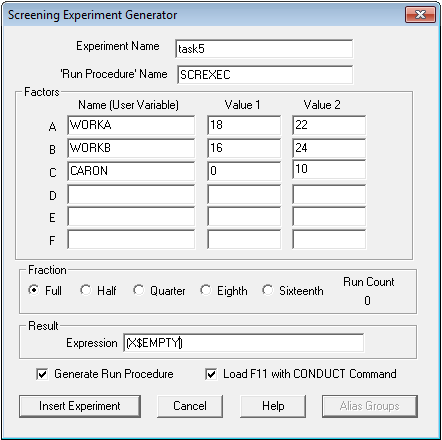
\includegraphics[scale=1]{res/pic001}
\caption{Органичения и результирующее выражение для Screening анализа}
\end{figure}

\lstinputlisting[language={},caption={Модель, сгенерированная средой для проведения Screening анализа}]{res/prog5.gpss}

Результаты моделирования представлены в листинге 14.

\lstinputlisting[language={},caption={Результаты моделирования для Screening анализа}]{res/prog5.report}

В отчёте мы видим, что ни одни из критериев даже близко не достиг критического значения F--распределения (7.71).

\newpage
\subsubsection{Сведение результатов дисперсионного анализа}

При проведении дисперсионного анализа, нами были проведены следующие исследования:
\begin{itemize}
\item однофакторный дисперсионный анализ (ОФДА);
\item двухфакторный дисперсионный анализ (ДФДА);
\item многофакторный дисперсионный анализ (МФДА). 
\end{itemize}

Для рассмотрения было выбрано два параметра из условий задачи и однин параметр, выбранный нами самостоятельно:
\begin{itemize}
\item WORKA -- время выпуска партии деталей в филиале A (20 $\pm$ 3 минуты по условиям задачи)
\item WORKB -- время выпуска партии деталей в филиале B (20 $\pm$ 5 минуты по условиям задачи)
\item CARON -- задержка между выпуском автомобилей на маршрут
\end{itemize}

Для каждого эксперимента была найдена статистика Фишера (F) и критическое значение, представленные в сводной таблице 1.

\begin{table}[htb]
	\begin{tabularx}{\textwidth}{|c|c|c|X|X|X|X|X|X|}
	\hline
	\multirow{2}{*}{Параметр} & \multicolumn{2}{c|}{Ограничения} & \multicolumn{2}{c|}{ОФДА} & \multicolumn{2}{c|}{ДФДА} & \multicolumn{2}{c|}{МФДА} \\ 
	\hhline{~--------}
	{} & Min & Max & F & $F_{0,05}$ & F & $F_{0,05}$ & F & $F_{0,05}$ \\ 
	\hline 
	WORKA & 18 & 22 & 0.158 & 7.71 & 1.643 & 5.32 & 1.000 & 7.71 \\ 
	\hline 
	WORKB & 16 & 24 & 1.000 & 7.71 & 0.246 & 5.32 & 1.000 & 7.71 \\ 
	\hline 
	WORKA + WORKB & {} & {} & {} & {} & 1.156 & 5.32 & {} & {} \\ 
	\hline 
	CARON & 0 & 10 & 2.431 & 7.71 & {} & {} & 1.000 & 7.71 \\ 
	\hline 
	\end{tabularx}
\caption{Cводная таблица результатов дисперсионного анализа}
\end{table}

Все критерии оказываются не значительными при данных ограничениях. При увеличении границ ограничений эффект становится значительно большим.

\newpage
\subsection{Оптимизация модели}

GPSS позволяет подобрать оптимальные параметры модели путём перебора её параметров. На рисунке 2 показаны ограничения (группа полей Movement), задаваемые для оптимизации.На ограничение  можно повлиять через задание величины Redirection Limit. Это значение устанавливает предел на количество изменений направления движения эксперимента по факторному пространству.

\begin{figure}[h!]
\centering
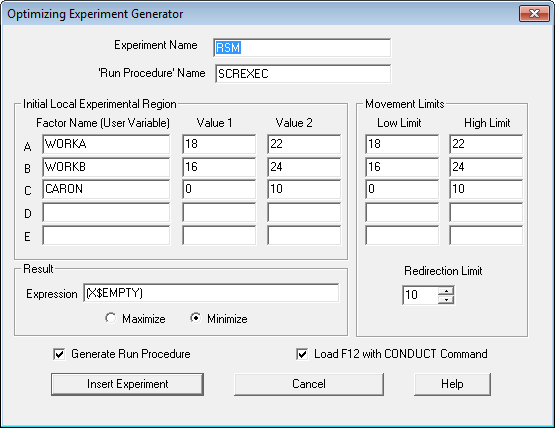
\includegraphics[scale=1]{res/pic002}
\caption{Органичения и результирующее выражение для оптимизации модели}
\end{figure}

В листинге 15 показан код, сгенинрированный средой GPSS

\lstinputlisting[language={},caption={Код для организации поиска оптимальных значений модели методом перебора}]{res/prog6.gpss}

Результаты некоторых наборов представлены в листинге 16. Стоит отметить, что большое число экспериментов выдаёт 0 для целевого значения. Так же наблюдаются ошибки, связанные с переполнением значений. Вцелом, можно говорить что модель и так достаточно оптимальна.

\lstinputlisting[language={},caption={Результат некоторых наборов при поиске оптимальных значений для модели}]{res/prog6.report}

\newpage
\section{Построение SAN-модели в Mobius}

Пакет Mobius позволяет построить расширенную (такими элементами как input/output gate) сеть Петри. На рисунке 3 разработана Atomic модель.

\begin{figure}[h!]
\centering
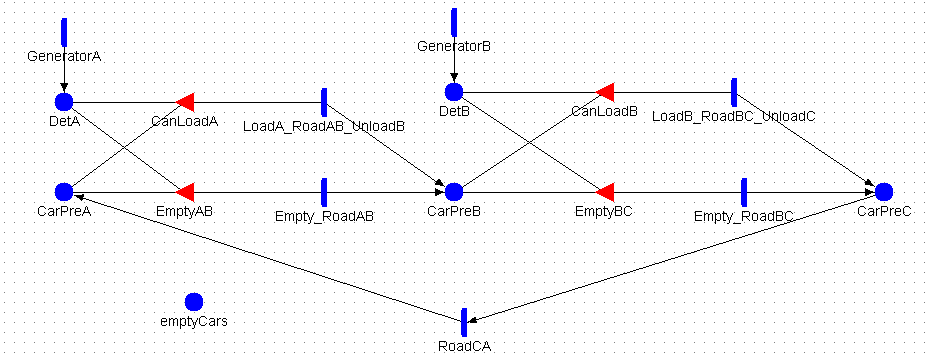
\includegraphics[scale=0.7]{res/pic003}
\caption{Atomic модель в абстракции SAN}
\end{figure}

Эту модель нужно читать с права на лево. Для начала, позиция \textbf{CarPredA}. В неё уже загружено 8 автомобилий, которые сразу выходят на линию, что отличается от модели в GPSS. Потом позиция \textbf{DetA}, в которую поступают детали каждые 20 $\pm$ 3 минуты (по нормальному распределению). Если есть готовая к загрузке машина и партия деталей, то через входной шлюз \textbf{CanLoadA} они отправляются в переход со временем \textbf{LoadA\_RoadAB\_UnloadB}, который эмулирует погрузку в филиале A (20 минут), дорогу до филиала B (30 минут) и потом разгрузку в филиале B (20 минут). Если партия не готова, то машина через входной шлюз \textbf{EmptyAB} отправляется к переходу со временем \textbf{Empty\_RoadAB} (20 минут). При этом увеличивается счётчик количества пустых прогонов в состоянии \textbf{emptyCars}. Это состояние фактически заменяет собой глобальную переменную, которая отказалась корректно работать в версии под Linux.

Аналогично происходит работа в филиале B -- готовые к погрузке машины находятся в позиции \textbf{CarPredB}, а детали филиала B копятся в состоянии \textbf{DetB}, куда поступаяют с частотой  20 $\pm$ 5 минут. После этого, можно либо через входной шлюз \textbf{CanLoadB} попасть в переход со временем \textbf{LoadB\_RoadBC\_UnloadC}, задача которого понятна из названия и занимает в сумме те же 20 + 30 + 20 минут, либо через шлюз \textbf{EmptyBС} попасть на 20 минут в \textbf{Empty\_RoadBC}, увеличив счётчик в \textbf{emptyCars}. С филиалом C всё проще, т.к. там может быть только разгрузка, а в моделе \textbf{RoadCA} показывает дорогу до филиала A.
\newpage
Помимо Atomic модели, проект в среде Mobius должен содержать Performance Variables Models (для вывода значений), Range Study (для управления параметрами моделирования, но в нашем случае не актуально) и Simulator (для проведения симуляции). Структура проекта представлена на рисунке 4.

\begin{figure}[h!]
\centering
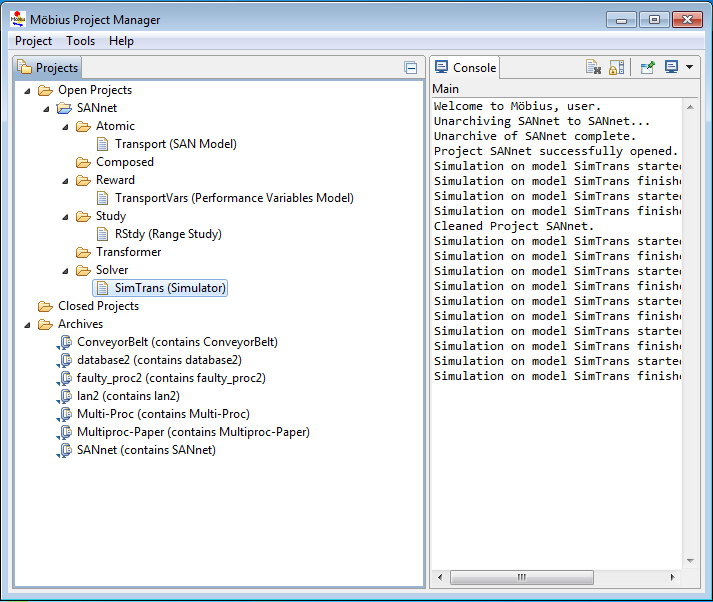
\includegraphics[scale=0.9]{res/pic004}
\caption{Проект в среде Mobius}
\end{figure}

Результаты моделирования представлены на рисунке 5. 

\begin{figure}[h!]
\centering
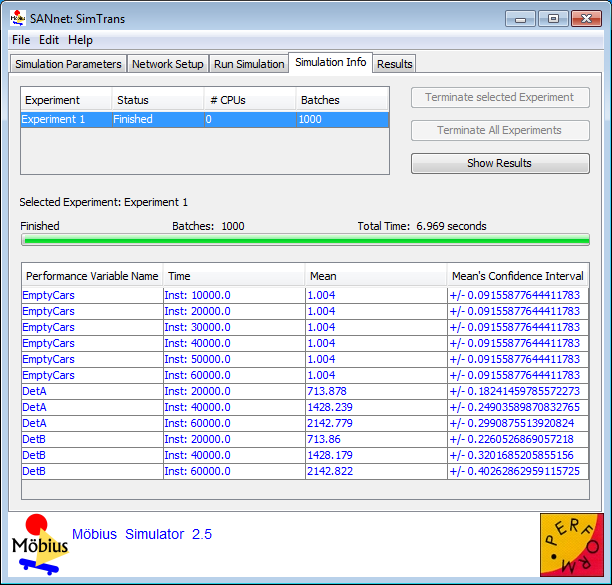
\includegraphics[scale=1]{res/pic005}
\caption{Симуляция задачи в среде Mobius}
\end{figure}

Можно заметить, что пустых машин практически нет (а те что есть, образовались в самом начале, когда сразу 8 штук вышло на линию до того, как филиалы завершили выпуск самой первой партии продукта). При этом в филиалах копится довольно много не транспортированной продукции, гораздо больше чем было показано в моделе на GPSS. Таким образом, модель может оказаться не вполне оптимальной с точки зрения эффективной работы системы, но отвечает требованию минимизации пустых прогонов, которое было поставлено в задаче.

Исходные коды достаточно грамоздки, по этой причине в отчёте они не приводятся, но доступны для изучения на GitHub: \url{https://github.com/SemenMartynov/SPbPU_CSSimulation}.


%\newpage
%\section{Аналитическая модель}

%Имя на руках модель в среде Mobius мы можем перейти к численному решению построенной модели путем %преобразования модели в Марковскую цепь и решения системы уравнений.

%Для этого требуется изменить закон распределения срабатывания переходов с нормального на экспоненциальный, добавим Transformer (для порождения Марковского процесса) и численный Solver, позволяющий получать решения без моделирования.





\newpage
\section{Построение YASPER-модели}

\newpage
\section*{Заключение}
\addcontentsline{toc}{section}{Заключение}

%------------------------------------------------------------------------------

\end{document}